\documentclass[../talk.tex]{subfiles}
\begin{document}

\begin{frame}{Automata theory}
    \begin{overlayarea}{\slidewidth}{\slideheight}

        Verification problems may be decidable if we consider \alert{automata} as input

        \vspace*{1em}

        \sonslide<2->%
        {%
            How to solve general verification problems?

            \begin{center}
                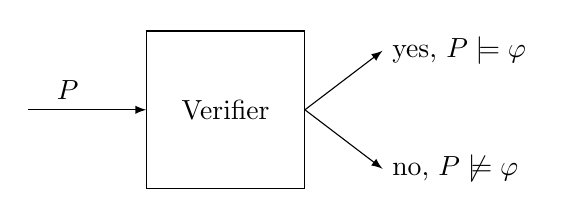
\begin{tikzpicture}
                    \node (origin) [coordinate] at (0.5,0) {};

                    \node (rect) at (2,0) [minimum width=2cm,minimum height=2cm, anchor=west,draw] {};

                    \node (yes) [coordinate] at (5,0.75) {};
                    \node (no) [coordinate] at (5,-0.75) {};
                    \path [->,>=latex]
                        (origin) edge (rect.west)
                        (rect.east) edge (yes)
                        (rect.east) edge (no)
                    ;

                    \node at (1,0.25) {$P$};
                    \node [right of=yes, node distance=0cm, anchor=west] {yes, $P \models \varphi$};
                    \node [right of=no, node distance=0cm, anchor=west] {no, $P \not\models \varphi$};
                    \node at (rect) {Verifier};
                \end{tikzpicture}
            \end{center}
        }

        \sonslide<3->%
        {%
            % \vspace*{-2em}
            \alert{Abstract} to an automaton first!

            \begin{center}
                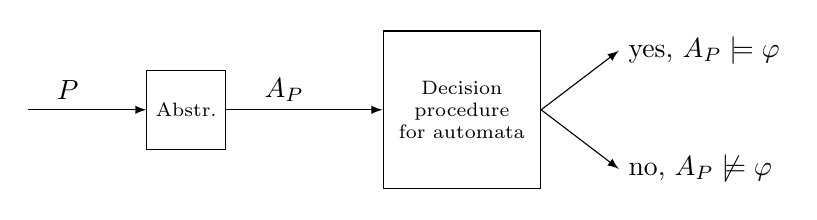
\begin{tikzpicture}
                    \node (origin) [coordinate] at (0.5,0) {};

                    \node (abstr) at (2,0) [minimum width=1cm, minimum height=1cm, anchor=west,draw] {};


                    \node (rect) at (5,0) [minimum width=2cm,minimum height=2cm, anchor=west,draw] {};

                    \node (yes) [coordinate] at (8,0.75) {};
                    \node (no) [coordinate] at (8,-0.75) {};
                    \path [->,>=latex]
                        (origin) edge (abstr.west)
                        (abstr.east) edge (rect.west)
                        (rect.east) edge (yes)
                        (rect.east) edge (no)
                    ;

                    \node at (1,0.25) {$P$};

                    \node at (3.75,0.25) {$A_P$};

                    \node [right of=yes, node distance=0cm, anchor=west] {yes, $A_P \models \varphi$};
                    \node [right of=no, node distance=0cm, anchor=west] {no, $A_P \not\models \varphi$};

                    \node [align=center, text width=1cm, font=\scriptsize] at (abstr) {Abstr.};
                    \node [align=center, text width=2cm, font=\scriptsize] at (rect) {Decision procedure for automata};
                \end{tikzpicture}
            \end{center}
        }
    \end{overlayarea}
\end{frame}

\end{document}
